\newpage
\section{Introduction}
Le projet choisi est celui du système de monitoring pour l'agriculture. Son but est de collecter des données de plusieurs capteurs répartis dans un champ, ce qui peut représenter une vaste surface et de les transmettre à l'agriculteur peu importe où il se trouve sur la parcelle.\\\\
Dans le cadre de ce projet nous allons utiliser deux capteurs SensorTag qui communiquent en Bluetooth Low Energy (BLE) pour collecter des informations sur l'humidité, la température et la luminosité. Les données sont ensuite transmises à un contrôleur via BLE qui va analyser les informations et déterminer s'il y a besoin de générer une alarme indiquant que les champs ont besoin d'être irrigués. Toutes les données collectées ainsi que l'alarme sont transmises au travers d'un réseau LoRaWAN qui permet de couvrir de longues distances.\\\\
Optionnelement nous pouvons implémenter une petite application permettant de voir les données et alarmes collectées par le réseau.\\\\
L'image ci-dessous représente notre système.
\begin{figure}[H]
	\begin{center}
		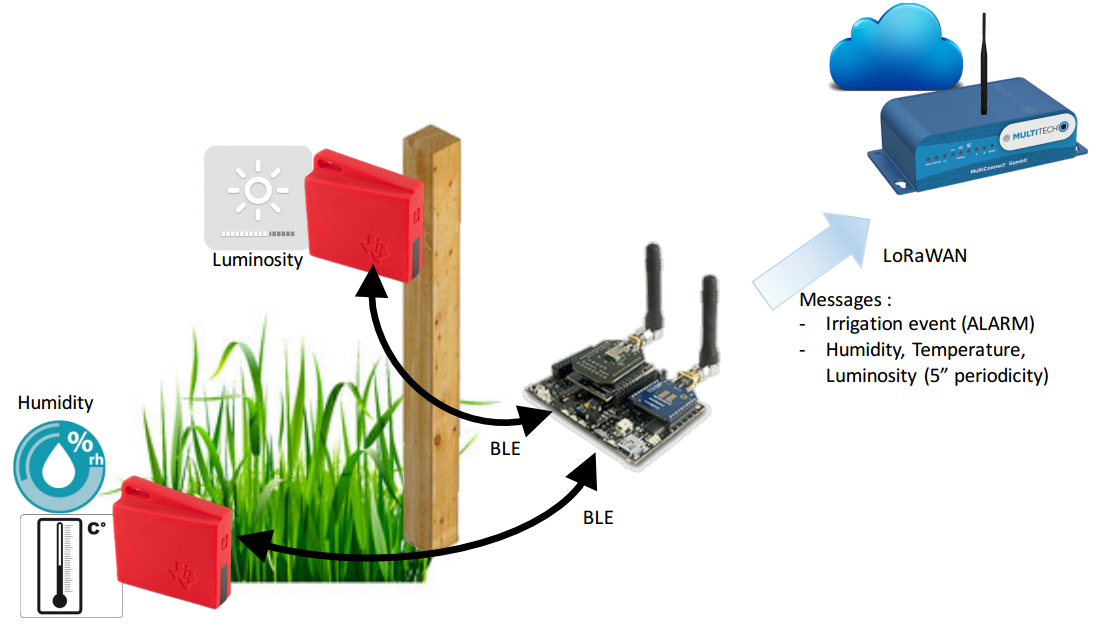
\includegraphics[width=17cm]{img/intro.png}
		\caption{Représentation du système}
		\label{intro}
	\end{center}
\end{figure}